%!tex root = ../main.tex

\section{Algorithm} \label{sec:algorithm}

%% Draft how this whole section should look like.
%% Then after that, spread these comments to their correct positions.
%%
% - Tell about this section 5
% - First, we want to answer to RQ1,  or how we can autom. detect the unsolvability of an LCL problem.
%   - For this, we first define what is solvability
%   - Then we define what is unsolvability (its complement)
%   - Lemma: LCL is not solvable in PN, if there exists a network that no algorithm can solve
%     - !Mention! that this is only one case where problem is unsolvable. There does not really have to be one network that is not solvable with any algorithm. The other option would be that for each algorithm, there is some network in which the problem is not solvable.
%   - Lemma: If LCL is not solvable in graph G, then the problem is also not solvable in any PN network N that has G as its underlying graph
%     - Proof: We proof by contradiction. We assume that PI is not solvable in G, and PI is solvable in some N that has G as its underlying graph. This means that there exists a valid labeling for N, therefore there must exist a valid labeling for G. This is contradicting with the assumption that PI is not solvable in G.
%   - We show the algorithm that finds graphs (counterexamples) and explain the algorithm.
% - Second, we show our theorem: if an LCL problem is unsolvable in the PN model, then the problem is also not solvable in constant time in the LOCAL model.
%   - We introduce some lemmas in the following subsections
%   - 

%
%
%




In this section, we will introduce the basic idea of an essential algorithm that we use in our implementation (discussed in section \ref{sec:implementation}).
The purpose of the algorithm is to find a proof that a given LCL problem $\Pi$ is impossible to solve in the PN model.
In case the algorithm detects the problem unsolvable, it outputs a multigraph as a result.
We need to prove that this multigraph is enough to show that the problem is not solvable in constant time ($\mathcal{O}(1)$) in the LOCAL model.
The proof is split into multiple parts under this section.
%Here we specifically allow PN networks to have multiple connections.
In Section \ref{sec:algorithm:from_multiple_to_simple} we show that the unsolvability of a problem $\Pi$ in PN networks (with multiple connections) implies that it is also impossible to solve $\Pi$ in \emph{simple} PN networks (without multiple connections).
Later in Section \ref{sec:algorithm:from_finite_to_infinite} we show that unsolvability of an LCL problem in finite networks implies the unsolvability of the problem in infinite trees.
Finally, in Section \ref{sec:algorithm:from_pn_to_local} we show that the unsolvability of $\Pi$ in PN networks implies that $\Pi$ is not solvable in constant time ($\mathcal{O}(1)$) in the LOCAL model.

First, we start with defining the meaning of solvability of an LCL problem.
%TODO These definitions and theorems might have a better place under section 2 background.
\begin{definition} \label{def:lcl_solvability}
    An LCL problem $\Pi$ is solvable in PN model, if and only if there exists a PN algorithm $A$ that finds a solution for $\Pi$ in all PN networks.
\end{definition}

We can define an alternative version of the Definition \ref{def:lcl_solvability} using contraposition.
\begin{definition} \label{def:lcl_solvability:contrapositive}
An LCL problem $\Pi$ is not solvable in PN model, if and only if there does not exist a PN algorithm $A$ that finds a solution for $\Pi$ in all PN networks.
\end{definition}

The Definitions \ref{def:lcl_solvability} and \ref{def:lcl_solvability:contrapositive} are equivalent. The latter definition might be more difficult to understand because of the contraposition, but we find it necessary to be shown as we find more fitting to discuss unsolvability rather than solvability.

%In the Table 2, we show an arbitrary LCL problem Pi that is unsolvable.
% Using Definition \ref{def:lcl_solvability:contrapositive}, we can see that for each network $A_i, 1 \leq i \leg m$, there exists some network $N_j, 1 \leg j \leg n$ where the algorithm cannot find a solution, denoted by value ``N''.

We have illustrated two examples of unsolvable LCL problems in Tables \ref{tbl:unsolvable_lcl:1} and \ref{tbl:unsolvable_lcl:2}, where the values ``Y'' (Yes) and ``N'' (No) answer to the question: \emph{can the algorithm in this row solve the problem in the network of this column?}
Value of ``Y/N'' indicates that the value does not matter for the purpose of the example.
In both examples, there are only finite number of networks and algorithms for the sake of simplicity.
In Table \ref{tbl:unsolvable_lcl:1}, the problem $\Pi$ is unsolvable, because there is at least one network for each algorithm, where the algorithm fails to solve the problem.
In Table \ref{tbl:unsolvable_lcl:2}, we show an example that is a special case of Definition \ref{def:lcl_solvability:contrapositive}.
The problem $\Pi'$ is also unsolvable, but this time \emph{no algorithm} can solve it in network $N'_{n'}$.

\begin{table}[H]
    \parbox{.45\linewidth}{
    \centering
        \begin{tabular}{c|ccccc}
        $\Pi$&$N_1$&$N_2$&$N_3$&$\cdots$&$N_n$ \\
        \hline
        $A_1$& N & Y/N & Y/N & $\cdots$ &  Y/N  \\
        $A_2$& Y/N & N & Y/N & $\cdots$ &  Y/N  \\
        $A_3$& Y/N & Y/N & N& $\cdots$ &  Y/N  \\
        $\vdots$&$\vdots$&$\vdots$&$\vdots$&$\ddots$&$\vdots$ \\
        $A_{m}$& Y/N & Y/N & Y/N & $\cdots$ &  N \\
        \hline
        \end{tabular}
    \caption{
        Unsolvable LCL problem $\Pi$.
        Each algorithm fails to solve $\Pi$ in at least some network, denoted by ``N'' (No).
    }
    \label{tbl:unsolvable_lcl:1}
    }
    \hfill
    \parbox{.45\linewidth}{
        \centering
        \begin{tabular}{c|ccccc}
        $\Pi'$&$N'_1$&$N'_2$&$N'_3$&$\cdots$&$N'_{n'}$ \\
        \hline
        $A'_1$& Y/N & Y/N & Y/N & $\cdots$ &  N \\
        $A'_2$& Y/N & Y/N & Y/N & $\cdots$ &  N \\
        $A'_3$& Y/N & Y/N & Y/N & $\cdots$ &  N \\
        $\vdots$&$\vdots$&$\vdots$&$\vdots$&$\ddots$&$\vdots$ \\
        $A'_{m'}$& Y/N & Y/N & Y/N & $\cdots$ &  N \\
        \hline
        \end{tabular}
    \caption{
        Unsolvable LCL problem $\Pi'$.
        Each algorithm fails to solve $\Pi'$ at least in network $N'_{n'}$ (the last column containing only values ``N'').
    }
    \label{tbl:unsolvable_lcl:2}
    }
\end{table}

Not every unsolvable LCL problem necessarily fall within the case shown in Table~\ref{tbl:unsolvable_lcl:2}.
Nevertheless, we are interested in it, because it seems more feasible to find a single network where all algorithms fail, in comparison to finding a network for each algorithm separately.
The special case is written as the following lemma:

\begin{lemma} \label{lem:lcl_unsolvability}
    An LCL problem $\Pi$ is not solvable in PN model, if there exists a PN network $N$ such that no PN algorithm $A$ can solve the $\Pi$ in $N$.
\end{lemma}
\begin{proof}
    Let $\Pi$ be an LCL problem.
    Let $N$ be a PN network such that no PN algorithm $A$ can solve $\Pi$ in $N$.
    Therefore, no PN algorithm $A$ can find a solution to $\Pi$ in all PN networks.
    According to Definition \ref{def:lcl_solvability:contrapositive}, the problem $\Pi$ is unsolvable.
\end{proof}

As the Lemma \ref{lem:lcl_unsolvability} shows us, to show that a problem $\Pi$ is unsolvable, it is enough to find a counterexample, a PN network $N$ in which the problem $\Pi$ cannot be solved.
To show that, it is enough to find an underlying graph $G$ of network $N$ in which the problem $\Pi$ cannot be solved.

\begin{lemma} \label{lem:problem_solvability_in_graphs}
    If a problem $\Pi$ is solvable in network $N$, then $\Pi$ also has a solution in its underlying graph $G$.
\end{lemma}
\begin{proof}
    Network $N$ is solvable, therefore it has a valid labeling.
    By the definition of underlying graph, $G$ has the same structure as network $N$, therefore it can be labeled exactly the same way as network $N$.
\end{proof}
\begin{corollary} \label{lem:problem_unsolvability_in_graphs}
    If a problem $\Pi$ is not solvable in graph $G$, then $\Pi$ is also not solvable in any PN network $N$ that has $G$ as its underlying graph.
\end{corollary}
\begin{proof}
This is a contraposition of Lemma \ref{lem:problem_solvability_in_graphs}.
\end{proof}

With the fact from Corollary \ref{lem:problem_unsolvability_in_graphs}, we can come up with an algorithm that automatically tries to find a counterexample graph:

\begin{algorithm}[H]
    \caption{Counterexample graph finder}
    \label{alg:counterexample_finder}
    \begin{algorithmic}[1] % The number tells where the line numbering should start
        \Require $1 \leq n_{low} \leq n_{high}$
        %\Require $\Pi$ is an LCL problem
        \Function{Find}{$n_{low},n_{high}, \Pi$} \Comment{Graph bounds $n_{low}$ and $n_{high}$, LCL problem $\Pi$} \label{alg:counterexample_finder:n_loop}
            \State $\Delta \gets \textsc{ActiveDegree}(\Pi)$ \label{alg:counterexample_finder:d_a}
            \State $\delta \gets \textsc{PassiveDegree}(\Pi)$ \label{alg:counterexample_finder:d_p}
            \For{$n\gets n_{low}, n_{high}$} \Comment{Iterate graph sizes from lowest to highest} \label{alg:counterexample_finder:n}
                \State $G_n \gets \textsc{GenerateGraphs}(n, \Delta, \delta)$ \label{alg:counterexample_finder:Gn}
                \ForEach{$g \in G_n$} \label{alg:counterexample_finder:g}
                    \If {\Not $\textsc{SolutionExists}(\Pi, g)$} \label{alg:counterexample_finder:solution_exists}
                        \State \Return $g$ \Comment{Return counterexample.}\label{alg:counterexample_finder:return_g}
                    \EndIf
                \EndFor
            \EndFor
            \State \Return \Comment{No counterexample found. Return nothing.} \label{alg:counterexample_finder:return_nothing}
        \EndFunction
    \end{algorithmic}
\end{algorithm}

The Algorithm \ref{alg:counterexample_finder} is designed to find the smallest counterexample graph for an LCL problem $\Pi$.
It starts from graphs with $n_{low}$ vertices and goes up to graphs with $n_{high}$ vertices.
We define $\Delta$ and $\delta$ to be the active and passive degree of the problem $\Pi$ respectively (rows \ref{alg:counterexample_finder:d_a} and \ref{alg:counterexample_finder:d_p}).
The variable for the current vertex count is called $n$ (row \ref{alg:counterexample_finder:n}).
For each graph with $n$ vertices, we generate all possible $(\Delta, \delta)$-biregular multigraphs with $\textsc{GenerateGraphs}(n, \Delta, \delta)$, and save the graphs into variable $G_n$ (row \ref{alg:counterexample_finder:Gn}).
The reason for generating only these types of graphs comes from the LCL formalism from Section \ref{sec:lcl_problems:biregular}.
Now, for each graph $g \in G_n$ (row \ref{alg:counterexample_finder:g}) we check if the given problem $\Pi$ has a solution using the function $\textsc{SolutionExists}(\Pi, g)$ (row \ref{alg:counterexample_finder:solution_exists}).
If a solution does not exist, we return the graph as a counterexample (row \ref{alg:counterexample_finder:return_g}).
In the case there are no counterexamples in graphs with $n_{low}$ to $n_{high}$ vertices, the algorithm returns nothing (row \ref{alg:counterexample_finder:return_nothing}).

Up to this moment, we have not discussed how the function \[ \textsc{GenerateGraphs}(n, \Delta, \delta) \] from row \ref{alg:counterexample_finder:Gn} generates the graphs, nor have we discussed how the function \[ \textsc{SolutionExists}(\Pi, g) \] from row \ref{alg:counterexample_finder:solution_exists} determines the existence of a solution.
These functions are implementation specific and in this section we assume that they exist as black boxes.
Later on Section \ref{sec:implementation} we introduce our implementations of these functions.
%First we would like to discuss about the $\textsc{GenerateGraphs}(n)$.
%As we know from Section \ref{}, %TODO refer to LCL section and make sure that it defines the LCL problems we are using here (LCL for (b,a)-biregular graphs).
%the LCL problems used in this thesis are defined for $(b,a)$-biregular graphs.
%Therefore we should not generate \emph{all} graphs but only the graphs of type $(b,a)$-biregular, where the degrees $b$ and $a$ are taken from the LCL problem $\Pi$.

As we said before, we use the LCL formalism from Section \ref{sec:lcl_problems:biregular}.
The formalism uses infinite $(\Delta, \delta)$-biregular trees, but the algorithm generates finite $(\Delta, \delta)$-biregular multigraphs.
In Section~\ref{sec:algorithm:from_multiple_to_simple}, we show that it is enough to find $(\Delta, \delta)$-biregular network with multiple connections, where the problem is unsolvable, because it implies that it is also unsolvable in some simple $(\Delta, \delta)$-biregular network.
This can be derived to work with graphs with Corollary~\ref{lem:problem_unsolvability_in_graphs}.
In Section~\ref{sec:algorithm:from_finite_to_infinite}, we show that if an LCL problem is unsolvable in finite connected $(\Delta, \delta)$-biregular graph $G$ with cycles, then it is also unsolvable in some infinite $(\Delta, \delta)$-biregular tree $G'$.
Finite $(\Delta, \delta)$-biregular graphs are always with cycles, when both $\Delta$ and $\delta$ are greater than 1, and this is in practice always the case, because we are not interested in biregular graphs with $\Delta=1$ or $\delta=1$ as they are trivial.

%TODO talk about graphs, why they are actually (b, a)-biregular multigraphs. Maybe this is explained by the fact that our LCL problems are defined for (b, a)-biregular.
%TODO talk about networks and graphs. In the above text they are refered as if they were the same thing.
%TODO Do we need to talk about trees and how these biregular multigraphs relate to them? 'Informally, the idea is to prove negative results for the case in which "we are in the middle of a very large tree, far away from the leaves".'

%After Sections \ref{sec:algorithm:from_finite_to_infinite} and \ref{sec:algorithm:from_multiple_to_simple}, we have completed discussing our algorithm, therefore after them, we have completed answering to Research question \ref{research_question:1}.
%Then, in Section \ref{from_pn_to_local}, we answer to Research question \ref{research_question:2}.

%We have divided the proofs into multiple theorems and grouped them under two different sections, Section \ref{sec:algorithm:from_multiple_to_simple} and Section \ref{sec:algorithm:from_pn_to_local}.
%The dependencies of theorems are shown in the Figure \ref{fig:algorithm:theorem_dependency}.
%
%\begin{figure}[H]
%    \centering
%    % https://tex.stackexchange.com/a/499577
%    \begin{tikzpicture}[]
%        \node (1) [] {Lemma \ref{lem:lcl_unsolvability:from_multiple_to_lift}};
%        \node (2) [right = of 1] {Lemma \ref{lem:lcl_unsolvability:from_klift_to_simple}};
%        \node (3) [below = of $(1)!0.5!(2)$] {Lemma \ref{lem:lcl_unsolvability:from_multiple_to_simple}};
%        \node (4) [below = of 3] {Lemma \ref{lem:lcl_unsolvability:5}};
%        \node (5) [below = of 4] {Theorem \ref{thm:lcl_unsolvability}};
%        %\node (4) [right = of mat2-2-1] {$\deg_G(4)=2$};
%        %\node (5) [right = of mat2-3-1] {$\deg_G(5)=2$};
%        \draw[<-] (1) edge (3);
%        \draw[<-] (2) edge (3);
%        \draw[<-] (3) edge (4);
%        \draw[<-] (4) edge (5);
%    \end{tikzpicture}
%    \caption{A dependency graph of the following theorems.\todo{Check that the picture is correct. Also check if it is even needed.}} \label{fig:algorithm:theorem_dependency}
%\end{figure}
%

\subsection{From multiple connection networks to simple networks} \label{sec:algorithm:from_multiple_to_simple}

In this section we show that if an LCL problem is not solvable in PN networks with multiple connections, then the problem is also not solvable in simple PN networks.
%We try to first prove a couple of related lemmas and at the end utilize the shown lemmas to show the theorem to be true.
\todo{Explain or show a figure of dependency of these lemmas???}

% Pi is unsolvable in multiple connection PN network N -> Pi is unsolvable in lift of N
\begin{lemma} \label{lem:lcl_unsolvability:from_multiple_to_lift}
If an LCL problem $\Pi$ is not solvable in PN network $N$, then it is also not solvable in any PN network $N'$ that is a lift of $N$.
\end{lemma}
\begin{proof}
    Let problem $\Pi$ have no solution in some PN network $N$.
    Then any algorithm $A$ produces a result that is invalid solution to $\Pi$ i.e. a local constraint is violated at least at some node $v$.
    Let $\phi: V' \rightarrow V$ be a covering map from $N'=(V', P', p')$ to $N=(V, P, p)$.
    Theorem 7.1. from the textbook \cite{HirvonenSuomelaDistAlg2020} shows that the nodes of $N'$ will have exactly the same state as their counterparts at $N$ for each time unit $t=0,1,...$
    Hence, if we run algorithm $A$ on both networks $N$ and $N'$, the local constraint violation at some node $v \in N$ also appears in all nodes $v' \in V'$ such that $\phi(v') = v$ i.e. the local constraint violations also appear in the covering network $N'$.
\end{proof}

% Network with multiple connections ----k-lift--->  simple network
\begin{lemma} \label{lem:lcl_unsolvability:from_klift_to_simple}
    If there is a PN network $N_2$ with multiple connections with $k$ being the highest count of multiple connections between any two nodes, then there exists a $k$-lift $N_1$ of $N_2$ such that $N_1$ is a simple PN network.
\end{lemma}
\begin{proof}
    Let $N_2=(V_2, P_2, p_2)$ be a PN network with multiple connections.
    Let $\operatorname{mul}(u, v)$ be the number of connections between any nodes $u, v \in V_2$.
    The highest count of multiple connections is $k=\max (\{ m(u, v) \mid u, v \in V_2\} )$.
    \footnote{\todo{Is the "maximum number of multiple connections" ambiguous? Does it appear as the highest count of parallel connections or as the total number of multiple connections in the network?}}
    Let $\operatorname{M}(x+hk) = x$ for all $x = 1, ..., k$ and $h\in \mathbb{N}$, for example $\operatorname{M}(1 + hk) = 1$ and $\operatorname{M}(k + hk) = k$.

    Let there be another network $N_1=(V_1, P_1, p_1)$ such that:
    \begin{itemize}
        \item For each $v \in V_2$, there are $k$ clones in $V_1$, namely the nodes $v_1, v_2, ..., v_k \in V_1$.
        Thus, the sizes $|V_1|$ and $k|V_2|$ are equal.
        %$V_1 = \{v_x: \forall v \in V_2, \forall x \in \{1, 2, ..., k\}\}$
        \item For each port $(v, i) \in P_2$, we have each port $(v_x, i) \in P_1$ where $x=1, 2, ..., k$.
        %% TODO remove these comments when this has been reviewed.
        %\item For each non-multiple connection $p_2((v, i)) = (u, j)$, we have connections $p_1((v_x, i)) = (u_x, j)$, where $x=1, 2, ..., k$.
        %\item For each multiple connections $p_2((v, i_a)) = (u, j_a)$ where $a = 1, 2, ..., \operatorname{mul}(u, v)$, we have $p_1((v_{x}, i_a)) = (u_{\operatorname{M}(x+a-1)}, j_a)$.
        %Note that the non-multiple connections are just a special case where $a$ is always $1$.

        \item For each connection $p_2((v, i_a)) = (u, j_a)$ where $a = 1, 2, ..., \operatorname{mul}(u, v)$, we have $p_1((v_{x}, i_a)) = (u_{\operatorname{M}(x+a-1)}, j_a)$.
        Note that if $\operatorname{mul}(u, v) = 1$, then $p_1((v_{x}, i_1)) = (u_{\operatorname{M}(x)}, j_1) = (u_{x}, j_1)$.
    \end{itemize}

    Now we show that there is a covering map $\phi: V_1 \rightarrow V_2$.
    Let $\phi(v_x) = v \in V_2$ for each $v_x \in V_1$ where $x=1, 2, ..., k$.
    We will show that $\phi$ is a covering map using the Definition \ref{def:covering_map}:
    \begin{itemize}
        \item By the definition of $\phi$, it is surjective.
        \item For each connection in $N_2$, we have $k$ similar connections in $N_1$, therefore degrees of each node are preserved.
        %% TODO remove these comments when this has been reviewed.
        %\item For each non-multiple connection $p_1((v_x, i)) = (u_x, j)$, where $x=1, 2, ..., k$, we have $p_2((v, i)) = (u, j)$.
        %From our definition of $\phi$ we can see that the mapping preserves port numbers and connections in non-multiple connections.
        %\item For each multiple connection $p_1((v_{x}, i_a)) = (u_{\operatorname{M}(x+a-1)}, j_a)$ we have
        %\begin{align*}
        %    p_2((\phi(v_{x}), i_a)) &= (\phi(u_{\operatorname{M}(x+a-1)}), j_a)\\
        %    \Leftrightarrow p_2((v, i_a)) &= (u, j_a)
        %\end{align*}
        %Both $(v, i_a)$ and $(u, j_a)$ are in $P_2$ and $p_2((v, i_a)) = (u, j_a)$, therefore for each multiple connection, the port numbers and connections are preserved.
        \item For each connection $p_1((v_{x}, i_a)) = (u_{\operatorname{M}(x+a-1)}, j_a)$ we have
        \begin{align*}
           p_2((\phi(v_{x}), i_a)) &= (\phi(u_{\operatorname{M}(x+a-1)}), j_a)\\
           \Leftrightarrow p_2((v, i_a)) &= (u, j_a)
        \end{align*}
        Both $(v, i_a)$ and $(u, j_a)$ are in $P_2$ and $p_2((v, i_a)) = (u, j_a)$, therefore for each connection, the port numbers and connections are preserved.
    \end{itemize}
    Each condition holds, hence the function $\phi$ is a covering map from $V_1$ to $V_2$
    therefore $N_1$ is a $k$-lift of $N_2$.

    We need to show that $N_1$ is a simple PN network i.e. it does not have multiple edges.
    %As we know, the non-multiple connections in $N_2$ are preserved in $N_1$ therefore we need to only look at the multiple connections of $N_2$ in more detail.
    There exists connections $p_1((v_{x}, i_a)) = (u_{\operatorname{M}(x+a-1)}, j_a)$ where $a=1, 2, ..., \operatorname{mul}(\phi(v_{x}),\phi(u_{\operatorname{M}(x+a-1)}))$.
    We see that nodes $u_{\operatorname{M}(x+a-1)}$ are distinct for all $a$ because $1 \leq a \leq \operatorname{mul}(\phi(v_{x}),\phi(u_{\operatorname{M}(x+a-1)})) \leq k$ and
    there are exactly k many "u" nodes in $V_1$, namely nodes $u_1, u_2, ..., u_k \in V_1$.
    Thus, for each node $v_x$, all connections from $v_x$ are mapped to distinct nodes, therefore $N_1$ is simple.

    The network $N_2$ is connected by the assumption (Section \ref{sec:underlying_graph}) but it might not be clear that $N_1$ is connected, thus we show next that this is the case.

    Let us look at all connections in $p_1$ and fix $a=1$.
    Then $p_1((v_{x}, i_a)) = (u_{\operatorname{M}(x+a-1)}, j_a)$
    $=p_1((v_{x}, i_1)) = (u_{x}, j_1)$.
    This shows that we can traverse from any node $w_x\in P$ to any other node $w'_x\in P$ only using nodes with subscript $x$.

    There are at least some nodes $u, v \in P_2$ such that $\operatorname{mul}(u,v) = k$, therefore we can traverse from any $u_x \in P_1$ to any $v_y \in P_1$ for any $x, y \in \{1, 2, ..., k\}$.
    Thus, $N_1$ is connected.
\end{proof}

%\begin{figure}[H]
% \centering
% \includegraphics[]{example-image-duck}
% \caption{\todo{Illustration of k-lift using Theorem \ref{lem:lcl_unsolvability:from_klift_to_simple}}}
% \label{fig:duck2}
%\end{figure}

\begin{figure}[H]
    \subcaptionbox{
      A PN network $N_2$ with multiple connections.
      \label{fig:algorithm:k-lift_proof_simple1:a}
    }%
      [.3\linewidth] {
      \centering
      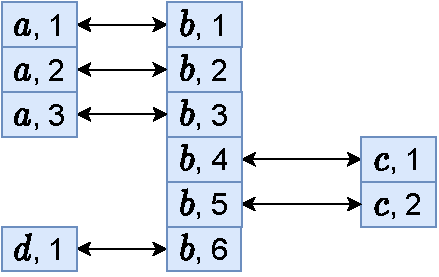
\includegraphics[scale=0.55]{diagrams/algorithm_k-lift_proof_simple_1.pdf}
    }%
    \subcaptionbox{
      A simple PN network $N_1$.
      \label{fig:algorithm:k-lift_proof_simple1:b}
    }%
      [.7\linewidth] {
      \centering
      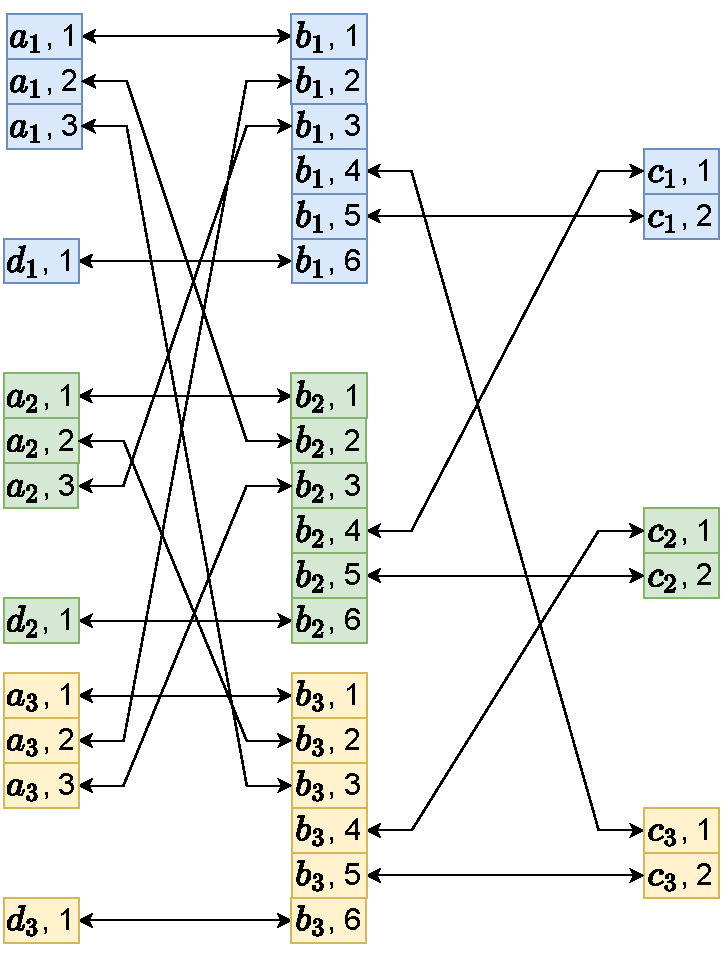
\includegraphics[scale=0.55]{diagrams/algorithm_k-lift_proof_simple_2.pdf}
    }
    \caption{The network $N_1$ is a 3-lift of the network $N_2$.
    }
    \label{fig:algorithm:k-lift_proof_simple1}
\end{figure}


%% This is more like an instruction on how to build the network, not a proof or is it?

    % Let $N=(V, P, p)$ be a PN network with multiple connections.
    % Let $m(u, v)$ be the number of connections between any nodes $u, v \in V$.
    % Let $k=\max {m(u, v) | u, v \in V}$ i.e. the maximum number of multiple connections.
    % \footnote{\todo{Is the "maximum number of multiple connections" ambiguous? Does it appear as the highest count of parallel connections or as the total number of multiple connections in the network?}}

    %Let's construct a new network $N'=(V', P', p')$ that consists of $k$ copies of $N$.
    %Initially the network $N'$ is not connected and therefore it is not a valid PN network but lets ignore this for now as the network gets valid soon as we alter it.
    %For each connection (v', j')
%
    %Let $\phi: V' \rightarrow V$ be a surjection such that for each node $v_i \in V'$ where $i=1, 2, ..., k$, $\phi(v_i) = v \in V$.
    %Next, we will swap the ends of connections such that the network becomes connected and
    %\todo{Complete this proof}
% Pi is unsolvable in multiple connection PN network N -> Pi is unsolvable in simple PN network N' (lift of N)
\begin{lemma} \label{lem:lcl_unsolvability:from_multiple_to_simple}
    If an LCL problem $\Pi$ is not solvable in PN network $N_2$ with multiple connections, then it is also not solvable in simple PN network $N_1$ that is a lift of $N_2$.
\end{lemma}
\begin{proof}
    Let us assume that an LCL problem $\Pi$ is not solvable in PN network $N_2$ with multiple connections.
    Theorem \ref{lem:lcl_unsolvability:from_klift_to_simple} shows that there exists a k-lift $N_1$ of $N_2$ such that $N_1$ is a simple PN network.
    Theorem \ref{lem:lcl_unsolvability:from_multiple_to_lift} shows that the problem $\Pi$ is also not solvable in network $N_1$.
    Therefore, we deduce that the problem $\Pi$ is not solvable in simple PN network $N_1$ that is a lift of $N_2$.
\end{proof}

\subsection{From finite to infinite} \label{sec:algorithm:from_finite_to_infinite}
Our algorithm outputs a finite connected $(\Delta, \delta)$-biregular multigraph with cycles, but in the LCL formalism, graphs are infinite $(\Delta, \delta)$-biregular trees.
With Lemma \ref{lem:lcl_unsolvability:from_multiple_to_simple}, we get simple networks from multiple connections, but we also need to show how unsolvability in finite graphs with cycles imply unsolvability in infinite trees.
%In the LCL formalism, the trees are infinite, so any naive approach of encoding these graphs would not suffice.
%Instead of generating infinite $(\Delta, \delta)$-biregular trees and finding some finite encoding for them, we can generate finite sized connected $(\Delta, \delta)$-biregular graphs with cycles.

\begin{lemma} \label{lem:from_finite_to_infinite}
    If an LCL problem $\Pi$ is unsolvable in finite connected $(\Delta, \delta)$-biregular graph $G$ with cycles, then it is also unsolvable in some infinite $(\Delta, \delta)$-biregular tree $G'$.
\end{lemma}
\begin{proof}
    Let us have a problem $\Pi$ that is unsolvable in finite connected $(\Delta, \delta)$-biregular graph $G=(V, E)$ with cycles.
    We construct an infinite $(\Delta, \delta)$-biregular tree $G'=(V', E')$.
    Let $v \in V$ be a seed node.
    We consider all possible non-backtracking walks from node $v$.
    Each walk is considered as a node of $G'$, and \emph{adjacent} walks are considered as adjacent nodes in $G'$.
    For example $v-a-b-c-a$ and $v-a-b-c-a-b$ are considered as adjacent walks, therefore they represent adjacent nodes in $G'$.
    Graph $G$ has cycles, therefore there are infinite walks of infinite length.
    Walks are non-backtracking, therefore the constructed graph $G'$ must be $(\Delta, \delta)$-biregular.
    We can see that $G'$ is a covering graph of $G$.
    Using Lemma \ref{lem:lcl_unsolvability:from_multiple_to_lift}, we deduct that the problem $\Pi$ must also be unsolvable in $G'$.
\end{proof}

%With Lemma \ref{lem:from_finite_to_infinite}, we can focus on finding finite connected $(\Delta, \delta)$-biregular graphs with cycles.

Now with Lemmas \ref{lem:lcl_unsolvability:from_multiple_to_simple} and \ref{lem:from_finite_to_infinite}, the output graphs from our algorithm imply the unsolvability in infinite $(\Delta, \delta)$-biregular trees.

\todo{How does this reflect to networks? The result is for graphs? Maybe refer to the Corollary \ref{lem:problem_unsolvability_in_graphs} and deduce unsolvability in networks. Actually, in the prior section "multi to simple", we have already networks. Take it into account.}


\subsection{From PN to LOCAL} \label{sec:algorithm:from_pn_to_local}

We begin by introducing the main theorem of this thesis:
\todo{
    Is it still the main theorem? It doesn't seem so.
    Maybe I should still leave it as it is as it would save me some time in the end.
    Changes take more time.
}

\begin{theorem} \label{thm:lcl_unsolvability}
    If an LCL problem is unsolvable in the PN model, then the problem is also not solvable in constant time in the LOCAL model.
\end{theorem}

\begin{lemma} \label{lem:lcl_unsolvability:5}
    If a problem is not solvable in infinite $(\Delta, \delta)$-biregular simple PN networks, then it is not solvable in constant ($\mathcal{O}(1)$) time in the LOCAL model.
    %TODO Make sure that the LOCAL model is explained under section 2. background.
    %TODO Make sure that the solving complexities (($\mathcal{O}(1)$) time) are explained under section 2. background.
\end{lemma}

Now we prove Theorem \ref{thm:lcl_unsolvability}:
\begin{proof}
    \todo{Complete this proof} %TODO Complete this proof

    Let us have an LCL problem $\Pi$ and a PN network $N$.
    Let us assume that the underlying graph of $N$ is infinite ($\Delta, \delta$)-biregular tree $G$, where problem $\Pi$ is not solvable.

    Theorem 3.3. from the paper \ref{DBLP:journals/siamcomp/NaorS95} shows that if there is a constant... \todo{}.

    \cite{DBLP:journals/siamcomp/NaorS95} "uses Ramsey theory arguments to prove that $\mathcal{O}(1)$-time LOCAL algorithms can be turned into ``order invariant'' $\mathcal{O}(1)$-time algorithms."

    This \cite{DBLP:journals/dc/GoosHS17} shows that ``Order invariant'' in trees are not stronger than PN algorithms in trees (Lemma 4) (Proof in Appendix A.2). PO is ``Port numbering + orientation'' which is very close to PN in biregular trees. Passive nodes have port numbering, therefore they can give an orientation of the edges.

\end{proof}


\subsection{Proving the theorem} \label{sec:algorithm:prooving_the_theorem}
\todo{With the current structure of Section \ref{sec:algorithm}, is this section needed? can't this proof be done in \ref{sec:algorithm:from_pn_to_local}?}
Now that all the groundwork has been done in the prior sections, we can prove Theorem \ref{thm:lcl_unsolvability}.
The proof is also our answer to Research Question \ref{research_question:2}.
\begin{proof}[Proof of Theorem \ref{thm:lcl_unsolvability}]
    Here is the proof.
    \todo{}
\end{proof}

\todo{rename all the names of theorems, lemmas and conjectures, that need renaming. }
